\documentclass[tikz,border=2pt]{standalone}
\usepackage{amsmath}
\usetikzlibrary{arrows.meta}
\begin{document}
% Two-station feedback network (Exercise 7.3.3 with gamma=1, alpha=0.5, beta_1=beta_2=0.25):
% traffic equations give lambda=(3,2); every arrow carries its flow rate lambda_j P_{ji},
% inflows at each station add up to lambda_i and the exit flow lambda_2 P_{20}=1 equals gamma.
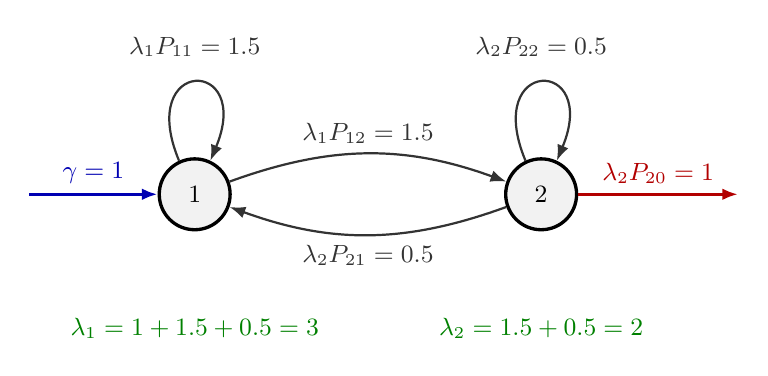
\begin{tikzpicture}[font=\small, >={Latex[length=2mm]},
  st/.style={circle, draw=black, very thick, fill=gray!10, minimum size=9mm}]
  \node[st] (s1) at (0,0) {$1$};
  \node[st] (s2) at (4.4,0) {$2$};
  % external arrivals
  \draw[->, very thick, blue!70!black] (-2.1,0) -- node[above] {$\gamma=1$} (s1.west);
  % routing flows
  \draw[->, thick, gray!40!black] (s1.20) to[bend left=20] node[above] {$\lambda_1P_{12}=1.5$} (s2.160);
  \draw[->, thick, gray!40!black] (s2.200) to[bend left=20] node[below] {$\lambda_2P_{21}=0.5$} (s1.340);
  \draw[->, thick, gray!40!black] (s1.115) .. controls (-0.75,1.75) and (0.75,1.75) .. (s1.65);
  \node[gray!40!black, anchor=south] at (0,1.62) {$\lambda_1P_{11}=1.5$};
  \draw[->, thick, gray!40!black] (s2.115) .. controls (3.65,1.75) and (5.15,1.75) .. (s2.65);
  \node[gray!40!black, anchor=south] at (4.4,1.62) {$\lambda_2P_{22}=0.5$};
  % exit
  \draw[->, very thick, red!70!black] (s2.east) -- node[above] {$\lambda_2P_{20}=1$} (6.9,0);
  % station totals
  \node[green!50!black, anchor=north] at (0,-1.45) {$\lambda_1=1+1.5+0.5=3$};
  \node[green!50!black, anchor=north] at (4.4,-1.45) {$\lambda_2=1.5+0.5=2$};
\end{tikzpicture}
\end{document}
